\chapter{Exploratory Analysis}
First part of the analysis is to explore the different attributes in the data in order to detect possible patterns or correlations. The exploratory analysis is also used to get an understanding of data and its behaviour. Hence, this chapter is about visualizing the different attributes focusing on their influence on heat consumption. 



%\begin{figure}[H]
%    \centering 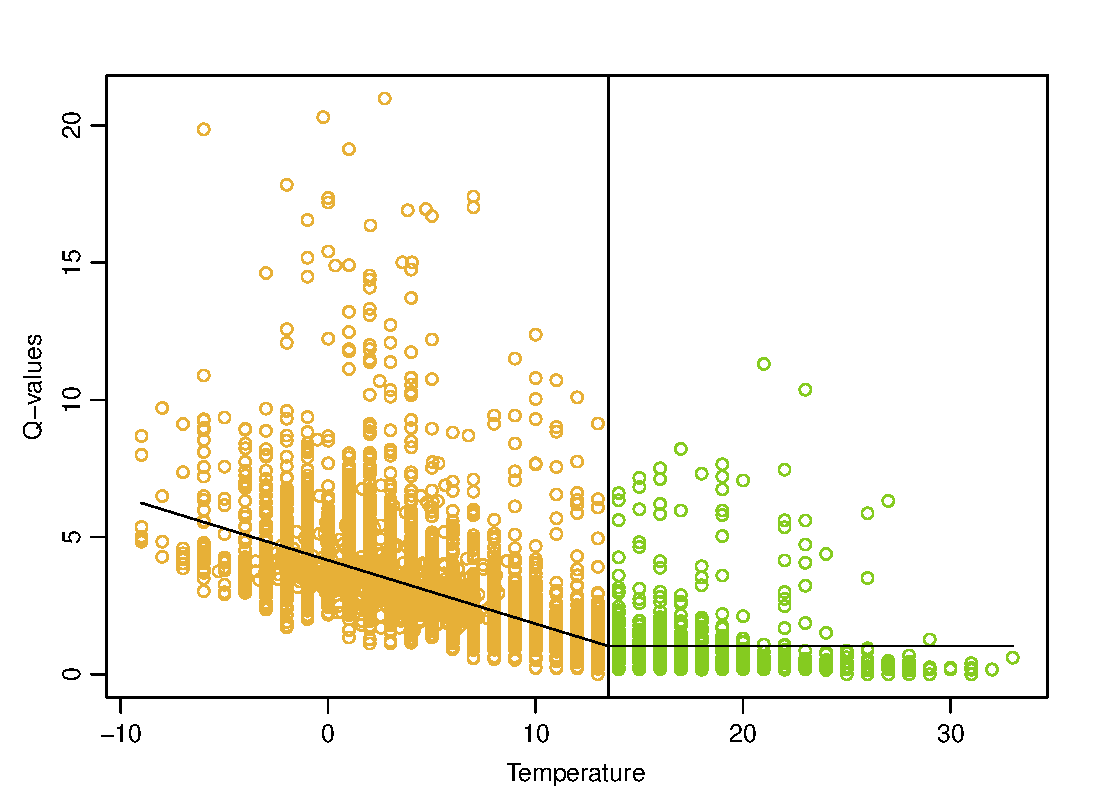
\includegraphics[width=1.\textwidth]{../../../figures/Consumption_H1.eps}
%    \caption{}
%    \label{fig: hej}
%\end{figure}